\documentclass{article}
\usepackage{amsmath}
\usepackage{tikz}
\begin{document}



\textbf{1a)} Queremos demostrar que $vw$ es un puente de $G \leftrightarrow$ $vw$ no pertenece a ningún ciclo de $G$. Probemos la ida y la vuelta:
\begin{itemize}


\item \textbf{ $vw$ es un puente de $G \rightarrow vw$ no pertenece a ningún ciclo de $G$}

Si $vw$ es un puente, quiere decir que removerla aumenta la cantidad de partes conexas. Observemos que si $vw$ perteneciese a un ciclo, entonces al sacarla, no estaríamos generando ninguna parte conexa nueva. Por virtud de ser ciclo, luego de remover a $vw$ ahora nos quedaría un camino simple, que sigue siendo claramente conexo. Luego, se sigue que $vw$ no pertenece a ningún ciclo de $G$.

\item \textbf{$vw$ no pertenece a ningún ciclo de $G \rightarrow vw$ es un puente de $G$}

Si $vw$ no pertenece a ningún ciclo, quiere decir que la arista es solo parte de un camino. Al remover la arista, necesariamente nos quedarán dos partes del camino, entre sí desconexas, luego $vw$ es un puente.
\end{itemize}
\begin{figure}[h]
    \centering
    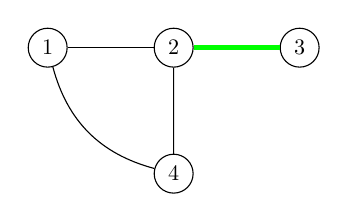
\begin{tikzpicture}[scale=0.8,transform shape]
        \node[circle,draw] (1) at (0,0) {1};
        \node[circle,draw] (2) at (2,0) {2};
        \node[circle,draw] (3) at (4,0) {3};
        \node[circle,draw] (4) at (2,-2) {4};
        
        \draw (1) -- (2);
        \draw[green,line width = 2pt] (2) -- (3);
        \draw (2) -- (4);
        
        \draw (1) to [bend right] (4);
    \end{tikzpicture}
    \hspace{1cm}
    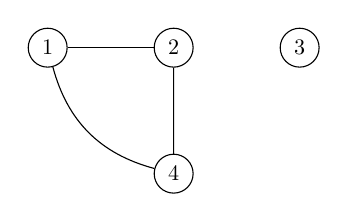
\begin{tikzpicture}[scale=0.8,transform shape]
        \node[circle,draw] (1) at (0,0) {1};
        \node[circle,draw] (2) at (2,0) {2};
        \node[circle,draw] (3) at (4,0) {3};
        \node[circle,draw] (4) at (2,-2) {4};
        
        \draw (1) -- (2);
        \draw (2) -- (4);
        \draw (1) to [bend right] (4);
    \end{tikzpicture}
    \caption{Grafo con y sin arista puente, se observa que el puente no podria pertenecer al ciclo}
\end{figure}
\textbf{b)}


\end{document}
